\renewcommand*{\arraystretch}{1.1}

\noindent\begin{tabularx}{\queryCardWidth}{|>{\queryPropertyCell}c|X|}
	\hline
	query & BI / 11 \\ \hline
%
	title & Unrelated replies \\ \hline
%
    pattern & \hfill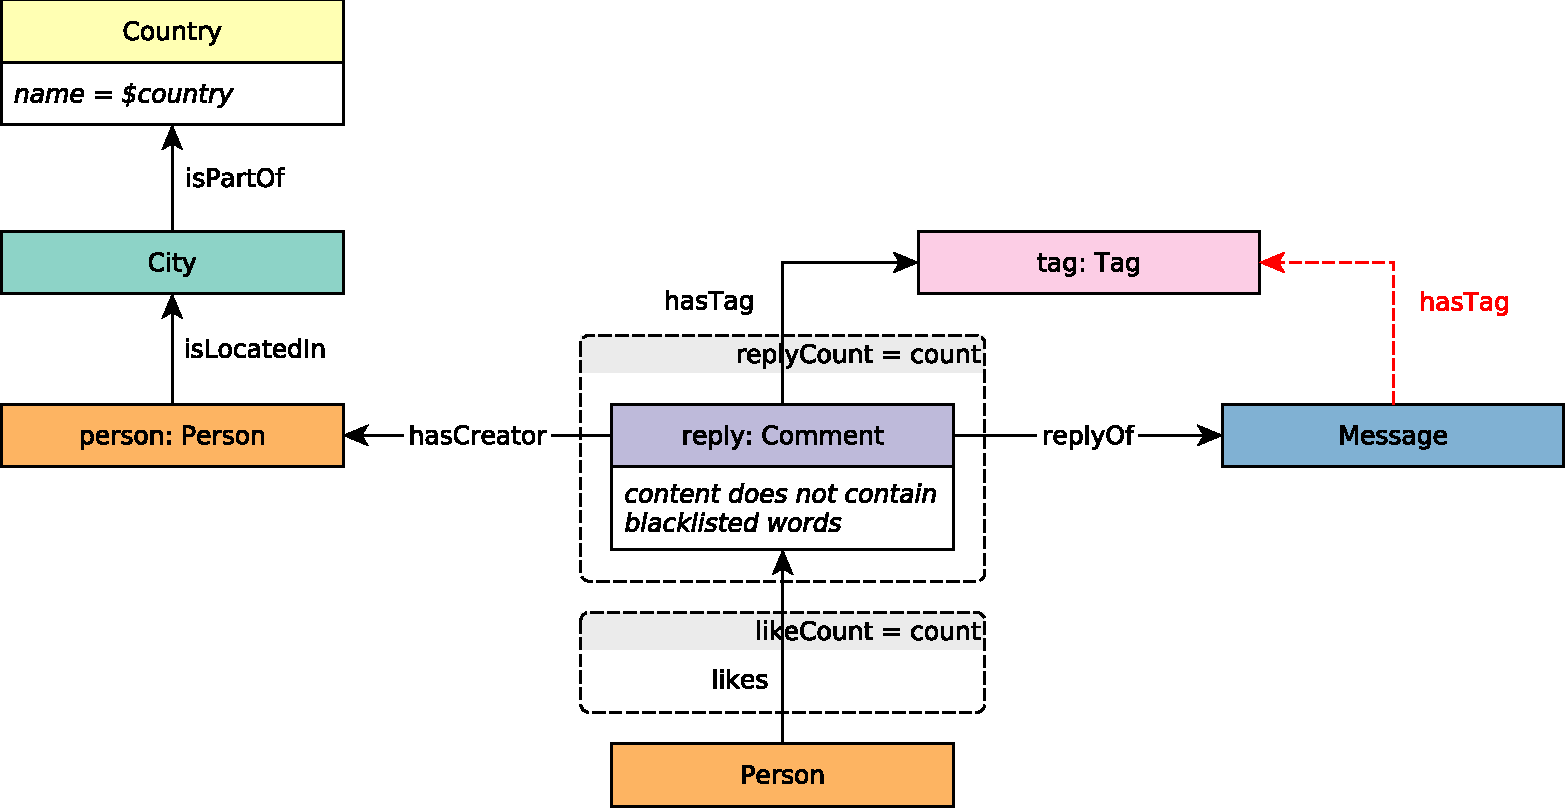
\includegraphics[scale=\patternscale,margin=0cm .2cm]{patterns/bi-read-11}\hfill\vadjust{} \\ \hline
%
	desc. & Find those Persons of a given country that replied to any Message, such
that the reply does not have any Tag in common with the Message {[}are
transitive replies considered or not? - SzG{]}. Consider only those
replies not containing any word from a given blacklist. For each Person
and valid reply, retrieve the Tags associated with the reply, and
retrieve the number of likes on the reply.
 \\ \hline
%
	
        group by &
        \multicolumn{1}{>{\raggedright}X|}{
            \varName{person.id}, 
            \varName{tag.name}
            } \\ \hline
	
%
	params &
	\innerCardVSpace{\begin{tabularx}{\attributeCardWidth}{|>{\paramNumberCell}c|>{\varNameCell}M|>{\typeCell}m{\typeWidth}|Y|} \hline
	\cellcolor{parameter} \color{white} \footnotesize $\mathsf{1}$ &country& 32-bit Integer &  \\ \hline
	\cellcolor{parameter} \color{white} \footnotesize $\mathsf{2}$ &blacklist& String[] &  \\ \hline
	\end{tabularx}}\innerCardVSpace \\ \hline
%
	
        result &
        \innerCardVSpace{\begin{tabularx}{\attributeCardWidth}{|>{\resultNumberCell}c|>{\varNameCell}M|>{\typeCell}m{\typeWidth}|>{\resultOriginCell}c|Y|} \hline
        $\mathsf{1}$ & person.id & 64-bit Integer &R&
                 \\ \hline
        $\mathsf{2}$ & tag.name & String &R&
                 \\ \hline
        $\mathsf{3}$ & countLikes & 32-bit Integer &A&
                The count of Likes to replies with that Tag. \\ \hline
        $\mathsf{4}$ & countReplies & 32-bit Integer &A&
                The count of replies with that Tag. \\ \hline
        \end{tabularx}}\innerCardVSpace \\ \hline
	
%
	sort        &
        \innerCardVSpace{\begin{tabular}{|>{\sortNumberCell}c|>{\varNameCell}l|>{\directionCell}c|} \hline
        $\mathsf{1}$ & countLikes & $\desc$ \\ \hline
        $\mathsf{2}$ & person.id & $\asc$ \\ \hline
        $\mathsf{3}$ & tag.name & $\asc$ \\ \hline
        \end{tabular}}\innerCardVSpace \\ \hline
	%
	limit & 100 \\ \hline
	%
	CPs &
	\multicolumn{1}{>{\raggedright}l|}{
	    \chokePoint{1.1}, 
	    \chokePoint{2.1}, 
	    \chokePoint{2.2}, 
	    \chokePoint{2.3}, 
	    \chokePoint{3.1}, 
	    \chokePoint{3.2}, 
	    \chokePoint{6.1}
	    } \\ \hline
	%
    %
\end{tabularx}
\queryCardVSpace